\chapter{Supersymmetry and the Standard Model}
\label{ch:SUSY}

The fundamental theory of particle physics, known as the Standard Model (SM) can predict precise interactions between the fundamental particles in our universe. With these predictions we are able to confirm processes, but there are some aspects of the universe that have not yet been explained. In this chapter, we will analyze the Standard model and the respective models that cannot be explained.

\section{The Standard Model}
\label{sec:SM}

After decades of theoretical and experimental research the SM has been developed into a theory that explains the Electromagnetic (EM), Strong, and Weak force. The SM has not yet been able to include Gravity into the theory. With the robust theoretical and experimental methods used in the SM, we have discovered new elementary particles and predicted others. 

\section{The Fundamental Particles}

 All the matter can be explained by three kinds of elementary particles: leptons, quarks, and gauge bosons. Each of these can be distinguished by various respective properties. The leptons and quarks are fermions which are particles that have half-integer spin. The leptons are particles that only interact with the EM force, while quarks interact with the EM and Strong force. The gauge bosons are the force carries for each respective force and have integer spin. 
 
 There are three generations of leptons and quarks which are differentiated by a charge $\pm e$, the charge of an electron. The leptons have three different charged particle: electron $(e)$, muon $(\mu)$, and tau $(\tau)$. With each charged particle having a corresponding neutrino $(\nu)$ of the same flavour, see fig \ref{SMParticles}. The quarks are also separated into three generations of doublets, the down-type $(-\frac{1}{3}e)$: down $(d)$, strange $(s)$, and bottom $(b)$ and up-type $(\frac{2}{3}e)$: up $(u)$, charm $(c)$, and top $(t)$. Each of the quarks has a color associated with it with is analogous to an electric charge, except there are three colors charges. 
 
\begin{figure}
 	\centering
	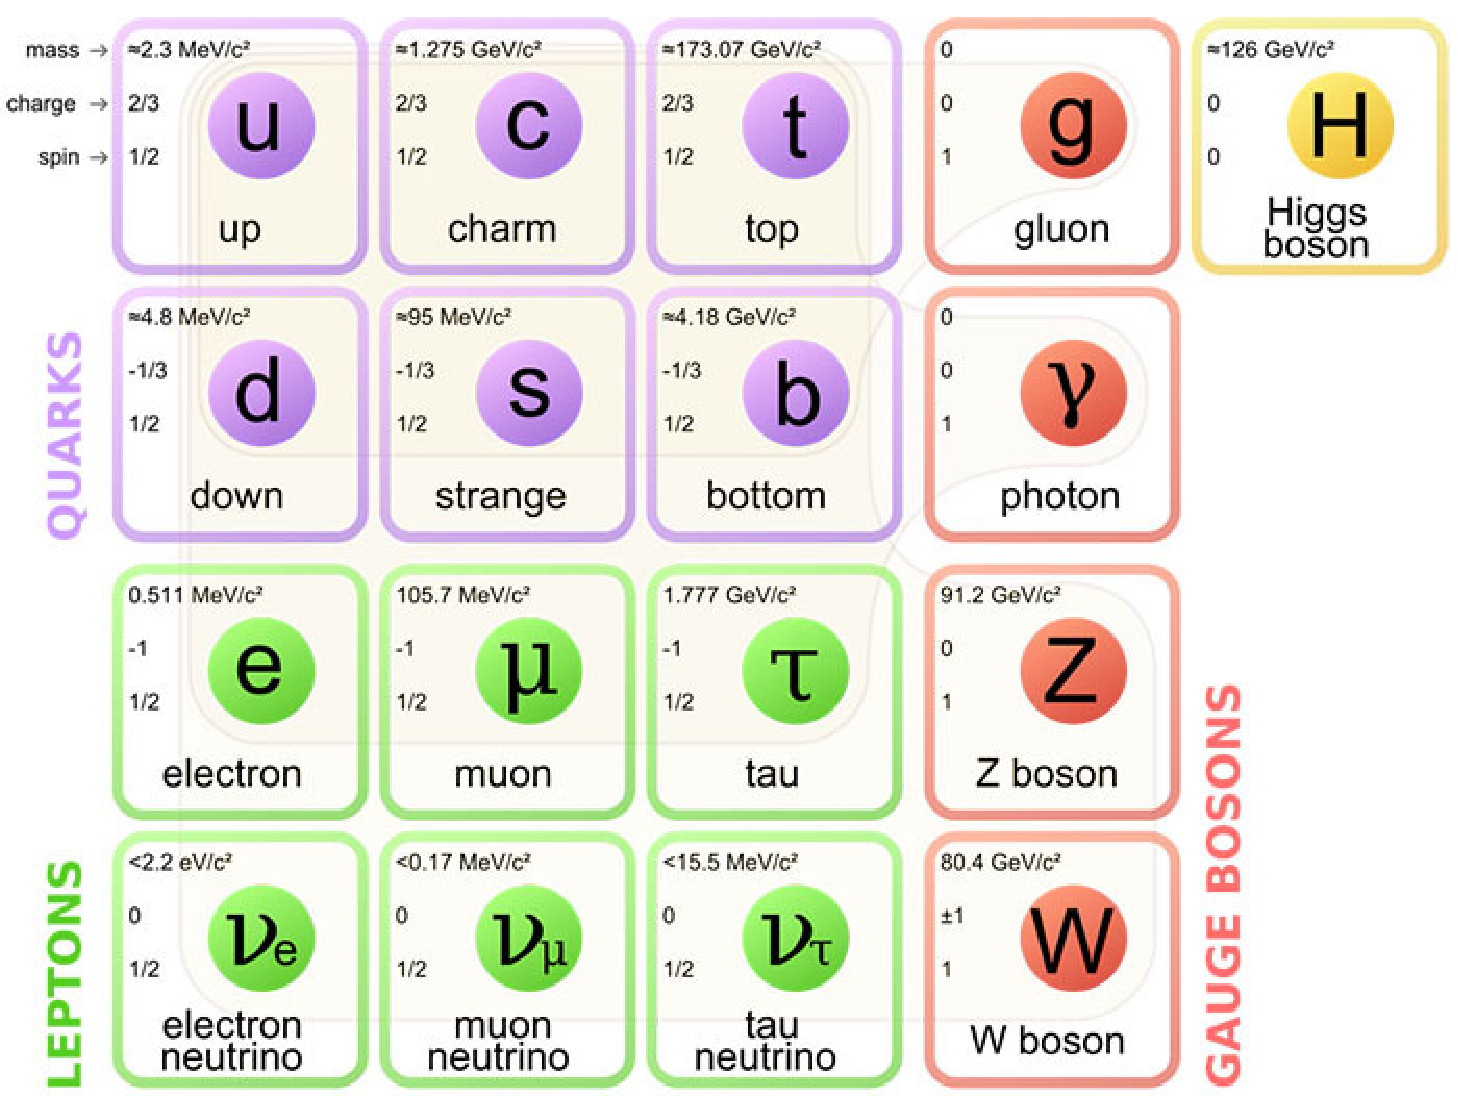
\includegraphics[scale=1,bb=0 0 300 300]{StandardModel.pdf}
 	\caption{The fundamental particle}
 	\label{SMParticles} 
\end{figure}
 
 \section{Quantum Field Theory}
 \label{QFT}
 
 Since many of the elementary particles in the standard model, we are mainly interested in the interactions of fermions. This is described by the Dirac equation, 
 
\begin{equation}
(i\gamma^\mu\partial_\mu-m)\psi(x)=0\label{Dirac},
\end{equation}

where $\gamma^\mu$ are matrices and are invariant under rotations of vector and spinor indices, $\partial_\mu$ is the partial derivative, $m$ is the mass of the particle, and $\psi(x)$ is the wave function of the particle. The combination of $\gamma^\mu\partial_\mu$ is a Lorentz-invariant differential operator. 
 

Why does the universe have to have this symmetry?
Universe hase the inverse square law for gravity and EM.

More symmetry allows for a simpler description of the values. 

\section{Fundamental Problems in the standard model}
\label{sec:Hierarchy}

Hierarchy problem?
Dark Matter?
Grand Unified Theory?

Support material for each of these unknowns and how SUSY can solve them. Fine Tuning

\section{Superpartners}
\label{sec:superpartners}

Initial assumption that every fermion has a boson partner and vice versa. These partners are exactly the same but differ by half integer spin. Changes Higgs mass divergence from quadratic to logrithmic (renormalizable)

Must be broken such that the masses of these partners are larger.

\subsection{Chirality}
\label{subsec:chiral}

Equal numbers of fermions and bosons. How does the spin change? 

\section{Minimal Supersymetric Standard Model}
\label{sec:MSSM}

Soft supersymetry breaking. 

\subsection{R Parity}
\label{subsec:rparity}

New conserved parameter known as R parity. With this is allows for a stable particle that is a dark matter candidate. Other consequences.

\section{Mass Spectrums}

Higgs boson corrections. spectrum of squarks. 






